\chapter{Lezione 14 - Cloud Computing - a confronto}

\FloatBarrier
\begin{figure}[H]
  \centering
  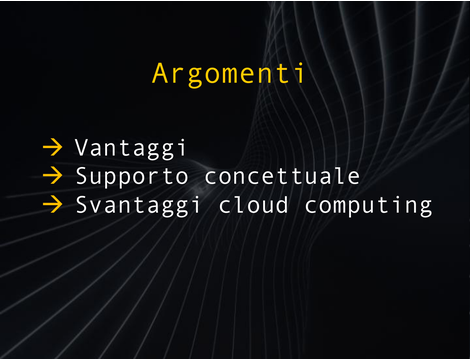
\includegraphics[width=0.50\textwidth,
                    trim=40 120 30 60, % L B R T
                    clip]
                    {images/Lez14_p01_fig_02}
  % \caption{Sommario}
  % \label{fig:Lez15_p06_fig_02}
\end{figure}
\FloatBarrier
\noindent

Argomenti trattati:

I vantaggi del cloud computing, il supporto concettuale,concetti, modelli, tecnologie a supporto della nascita e all'operatività di questo modello.
Inoltre nella parte conclusiva alcuni svantaggi, i problemi che possono insorgere con l'adozione di questo modello di erogazione.

\section{Vantaggi}

\FloatBarrier
\begin{figure}[H]
  \centering
  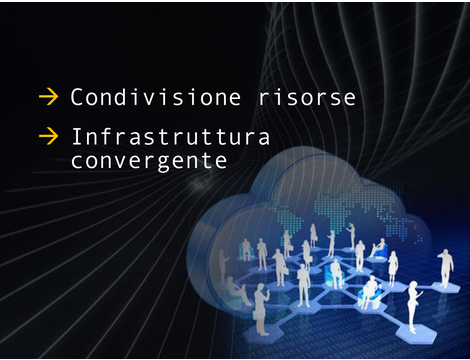
\includegraphics[width=0.50\textwidth,
                    trim=40 160 40 60, % L B R T
                    clip]
                    {images/Lez14_p01_fig_04}
  % \caption{Sommario}
  % \label{fig:Lez15_p06_fig_02}
\end{figure}
\FloatBarrier
\noindent

I vantaggi si includono in due classi, la condivisione delle risorse e l'infrastruttura convergente ovvero il modo di gestire le risorse.

\subsection{Condivisione delle risorse}

\FloatBarrier
\begin{figure}[H]
  \centering
  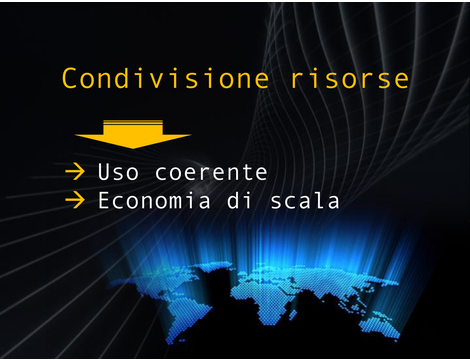
\includegraphics[width=0.50\textwidth,
                    trim=40 120 40 60, % L B R T
                    clip]
                    {images/Lez14_p01_fig_05}
  % \caption{Sommario}
  % \label{fig:Lez15_p06_fig_02}
\end{figure}
\FloatBarrier
\noindent

La condivisione delle risorse permette un uso coerente.
Abbiamo visto che il modello cloud è basato sulla clusterizzazione, sul raggruppamento di una vasta varietà di risorse di calcolo, di memorizzazione, di connessione, risorse fisiche e risorse software, che possano essere richieste per il confezionamento, per l'erogazione di un servizio.
Per il confezionamento di un servizio penso alla situazione in cui l'utente chiede un'applicazione, che gli sia risolta una necessità computazionale senza sapere quali sono le risorse effettivamente necessarie, la loro configurazione e la loro quantità.

Questo modello permette di spostare sul fornitore,  sull'erogatore, sul gestore del servizio questo compito di selezionare le risorse necessarie secondo la qualità necessaria all'erogazione e la quantità per l'impegno computazionale richiesto dal servizio voluto dal cliente o dall'utente.

Questo modo di gestire favorisce l'economia di scala.
L'economia di scala è favorita principalmente dalla virtualizzazione delle risorse fisiche che permettono di dare all'utente una visione differente da quella fisica, o meglio qualitativamente può essere identica, ma come quantità possiamo offrire risorse anche superiori, una memoria superiore gestita virtualmente in una memoria fisica più limitata, potenza di calcolo differenziata, di fatto vincolata alle risorse fisiche ma in maniera trasparente all'utente, una larghezza di banda potenzialmente molto alta per l'utente, dipendente poi a livello fisico sia dalla larghezza di banda fisica permessa dai canali di comunicazione, sia dal effettivo traffico che deve essere sostenuto.

\subsection{Infrastruttura convergente}

\FloatBarrier
\begin{figure}[H]
  \centering
  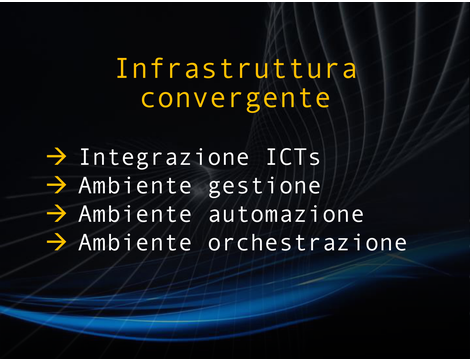
\includegraphics[width=0.50\textwidth,
                    trim=40 80 40 40, % L B R T
                    clip]
                    {images/Lez14_p01_fig_06}
  % \caption{Sommario}
  % \label{fig:Lez15_p06_fig_02}
\end{figure}
\FloatBarrier
\noindent

L'infrastruttura convergente è uno degli elementi fondanti di questo modello, è l'integrazione delle ICT.
L'infrastruttura convergente che è una caratteristica del modello cloud computing si riferisce alla possibilità di selezionare e integrare risorse di calcolo non in dipendenza diretta dalla richiesta dell'utente ma per soddisfare la sua esigenza, ovvero ribadisco che l'utente non fa una richiesta di risorse, fa una richiesta di servizi o presenta un problema che viene risolto dal sistema che seleziona le tecnologie in tipo e quantità necessaria per soddisfare quella richiesta.

Questo naturalmente richiede la disponibilità di risorse fisiche ma anche un ambiente di gestione per la misurazione ma anche per l'allocazione e per il rilascio delle varie risorse.

Questo tipo di gestione non può essere fatto in maniera interattiva perché già la virtualizzazione e la gestione di risorse multiple producono un sovraccarico di lavoro gestionale rispetto al puro carico di lavoro computazionale e di trasferimento dati necessario per l'esecuzione del servizio; questa gestione deve essere automatizzata, l'ambiente di automazione provvede automaticamente al controllo e al monitoraggio nel senso della gestione, la supervisione delle risorse necessarie utilizzate in un dato istante dai servizi, dalle procedure di automazione dei servizi che sono in atto nel sistema cloud.

Un ambiente di orchestrazione  perché le risorse devono essere selezionate, stabilito il loro ruolo e descritto il loro comportamento, deve essere definita una regia perché le varie risorse che possono essere fisiche o software, i servizi che dovranno contribuire alla risoluzione, al soddisfacimento della richiesta o del problema dell'utente dovranno essere coordinate e quindi lasciate a un'esecuzione automatica programmata.

\subsection{Infrastruttura convergente}

\FloatBarrier
\begin{figure}[H]
  \centering
  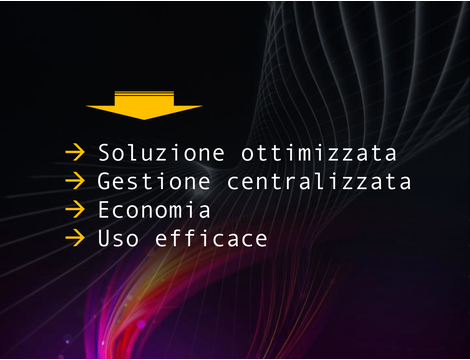
\includegraphics[width=0.50\textwidth,
                    trim=40 80 40 60, % L B R T
                    clip]
                    {images/Lez14_p02_fig_01}
  % \caption{Sommario}
  % \label{fig:Lez15_p06_fig_02}
\end{figure}
\FloatBarrier
\noindent

Questo permette di ottenere soluzioni ottimizzate sulle necessità dell'utente e anche ottimizzate per quanto riguarda i costi, almeno per quanto riguarda le esigenze delle varie computazioni attivate.
Inoltre la gestione viene centralizzata, non nello stesso luogo geografico, ma sotto la gestione dello stesso middleware.

Il sistema di gestione del cloud provvederà al coordinamento delle variabili in campo.
L'economia è data dal fatto che per il soddisfacimento del servizio richiesto l'utente non ha bisogno di acquisire risorse fisiche sovrabbondanti, nel senso che non sempre quando utilizziamo un applicativo, un sistema su un calcolatore, il calcolatore verrà utilizzato a pieno; questo significa che per la parte di sistema che noi abbiamo acquistato ci sarà un sottouso, con un costo per nulla, per una macchina che non lavora, per una memoria sovrabbondante utilizzata, un parco dischi, una memoria che non viene utilizzata a pieno, uno spazio dedicato a un DBMS non utilizzato a pieno, ecco che noi abbiamo acquisito memoria, abbiamo acquisito spazio che non utilizziamo.

Questo discorso vale anche per le figure funzionali, per gestire un parco macchine, per gestire delle risorse di calcolo, per gestire della connessione, aggiornare il software necessario servono figure funzionali che magari non vengono sfruttate a pieno dalla organizzazione.

L'uso efficace è dato dal fatto che le risorse sono utilizzate al massimo con vantaggio del fornitore dei servizi e vantaggio per l'economia del servizio per i clienti, per gli utenti dei servizi cloud.

\subsection{Orchestrazione}

\FloatBarrier
\begin{figure}[H]
  \centering
  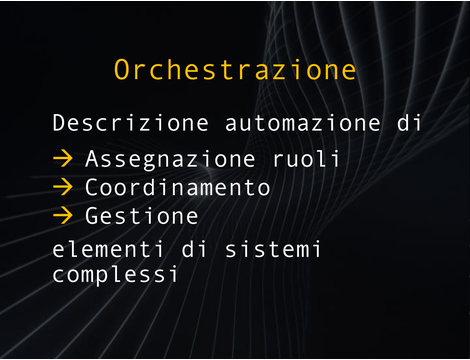
\includegraphics[width=0.50\textwidth,
                    trim=40 40 40 40, % L B R T
                    clip]
                    {images/Lez14_p02_fig_02}
  % \caption{Sommario}
  % \label{fig:Lez15_p06_fig_02}
\end{figure}
\FloatBarrier
\noindent

Rivediamo il concetto di orchestrazione che è basilare per il cloud; è una descrizione dell'automazione nell'assegnazione dei ruoli delle varie risorse, sia fisiche che software  ma può essere un servizio che va selezionato come componente di un servizio più complesso che andrà a costituire.

Il coordinamento tra questi vari elementi, tra i vari attori che sono orchestrati, deve essere descritto, stiamo parlando di descrizione delle modalità di selezione degli attori in gioco e del loro ruolo e della conduzione dell'intera attività.

La gestione viene prevista in questa descrizione, come i vari attori dovranno interagire durante lo svolgimento della attività.
Questo permette di costituire elementi di sistemi complessi, di organizzare elementi in sistemi più complessi.

\FloatBarrier
\begin{figure}[H]
  \centering
  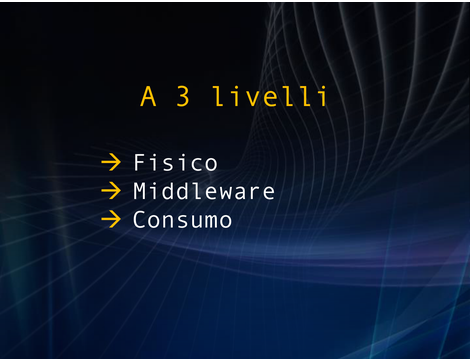
\includegraphics[width=0.50\textwidth,
                    trim=40 100 40 60, % L B R T
                    clip]
                    {images/Lez14_p02_fig_03}
  % \caption{Sommario}
  % \label{fig:Lez15_p06_fig_02}
\end{figure}
\FloatBarrier
\noindent

Nel cloud vi sono tre livelli di orchestrazione o in altri termini l'orchestrazione agisce a tre livelli.
Il livello fisico, quello delle risorse; per risorse pensiamo alle risorse fisiche, ma dobbiamo considerare che nel modello cloud tutte le risorse fisiche sono virtualizzate e offerte nella loro immagine virtuale.
Quindi quando parliamo di risorse fisiche ci rivolgiamo alla macchina virtuale, alla memoria virtuale, all'accesso virtuale alla rete; manteniamo sempre come intermediario il livello di virtualizzazione e delle risorse.

L'orchestrazione agisce anche a livello middleware, a livello intermedio e permettono l'erogazione delle risorse, il coordinamento delle risorse secondo questo specifico modello.

Il livello di consumo è il livello dei servizi, il livello dove interagisce direttamente il consumatore e l'utente, dove gli elementi, gli attori in gioco sono effettivamente i servizi, quindi attività autonome rilevanti per lo scopo dell'utente che possono però essere unite e coordinate come componenti di un servizio più complesso.

\FloatBarrier
\begin{figure}[H]
  \centering
  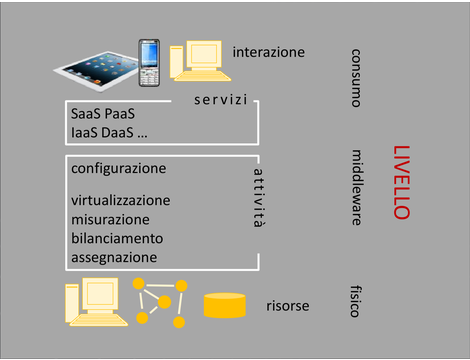
\includegraphics[width=0.60\textwidth,
                    trim=40 20 40 20, % L B R T
                    clip]
                    {images/Lez14_p02_fig_04}
  % \caption{Sommario}
  % \label{fig:Lez15_p06_fig_02}
\end{figure}
\FloatBarrier
\noindent

Vediamo in questa slide una sintesi grafica del comportamento della orchestrazione in un modello cloud.

Abbiamo il primo livello fisico con le varie risorse, risorse di calcolo, modelli di organizzazione dei dati o reti di calcolatori, strumenti per la connessione, router piuttosto che strumenti per la protezione delle reti da attacchi quali firewall, abbiamo risorse per la memorizzazione, abbiamo tutte le risorse di base su cui agiscono le attività gestionali del cloud computing. 

Abbiamo quelle gestionali quali la misurazione dell'uso delle varie risorse richieste dai servizi e dagli applicativi che svolgono; il bilanciamento cioè il controllo ed uso delle singole risorse che siano risorse di calcolo, di connessione o di utilizzo delle memorie perché il sistema automaticamente capisca quando una risorsa sta arrivando a saturazione e quindi cerchi una risorsa con disponibilità e possa assegnarla in maniera dinamica al determinato servizio. Quando la risorsa non è più necessaria viene rilasciata, non rimane di proprietà di quel processo ma viene assegnata a un nuovo servizio, a una nuova computazione.

Abbiamo un'attività di configurazione che permette l'interazione dell'utente, questo è l'unico punto in cui l'utente può intervenire con le sue interfacce, per configurare il servizio a livello che gli è permesso; ricordiamo che l'utente a seconda del servizio, application, software as a service, infrastructure as a service, platform as a service, data as a service, può intervenire a configurare il sistema a un livello specifico per quel dato servizio.

Al livello di consumo intervengono i servizi erogati secondo il modello Software as a Service, Platform as a Service, Data as a Service e così via, con la possibilità di accesso, di interazione da client ospitati da device di tipo differente, di tipo molto vario.

Spunto di riflessione: ripensate ai vantaggi offerti dal modello cloud.

\section{Supporto concettuale}

\FloatBarrier
\begin{figure}[H]
  \centering
  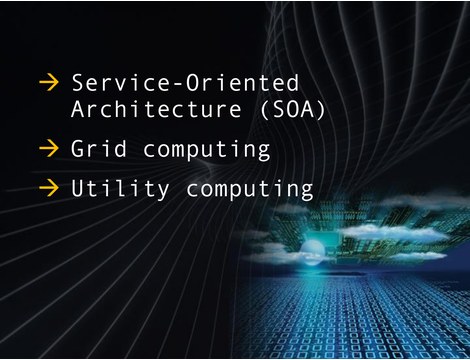
\includegraphics[width=0.50\textwidth,
                    trim=40 120 40 40, % L B R T
                    clip]
                    {images/Lez14_p03_fig_01}
  % \caption{Sommario}
  % \label{fig:Lez15_p06_fig_02}
\end{figure}
\FloatBarrier
\noindent

In questa parte vedremo tre concetti, tre modelli di organizzazione, tre modelli di calcolo, di gestione delle risorse di calcolo che hanno una rilevanza sia nel supporto logico sia nella nascita del modello di erogazione dei servizi chiamato cloud computing.

Rivediamo il service oriented architecture (SOA), paradigma orientato alla progettazione di architetture di sistema orientate al servizio, quindi ha elementi autonomi rispetto agli altri elementi in gioco che svolgano attività di interesse per l'utente.

Vedremo il Grid Computing che è un modello di architettura di sistemi di calcolo che è molto simile al cloud.

Terzo Utility Computing che è un approccio all'organizzazione delle risorse orientato all'utilità, orientato allo scopo dell'utente.

Quindi capiamo come questi tre concetti intervengano a completare il quadro concettuale del modello cloud computing.

\subsection{Service Oriented Architecture}

\FloatBarrier
\begin{figure}[H]
  \centering
  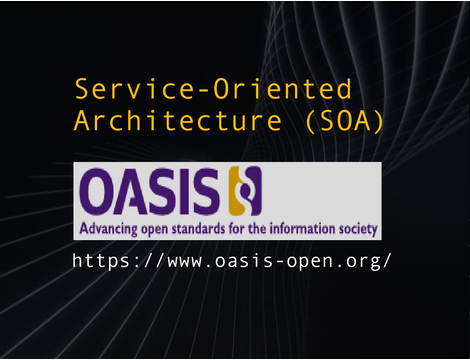
\includegraphics[width=0.50\textwidth,
                    trim=40 60 40 40, % L B R T
                    clip]
                    {images/Lez14_p03_fig_02}
  % \caption{Sommario}
  % \label{fig:Lez15_p06_fig_02}
\end{figure}
\FloatBarrier
\noindent

E' stato definito dall'OSIS, è un consorzio non profit con sede negli Stati Uniti costituito da 5.000 partecipanti, da 600 organizzazioni in più di 65 paesi nel mondo; si occupa dello sviluppo di standard legati alle tecnologie di web services, che sono le tecnologie molto utilizzate per la realizzazione del paradigma del modello architetturale orientato ai servizi.

\FloatBarrier
\begin{figure}[H]
  \centering
  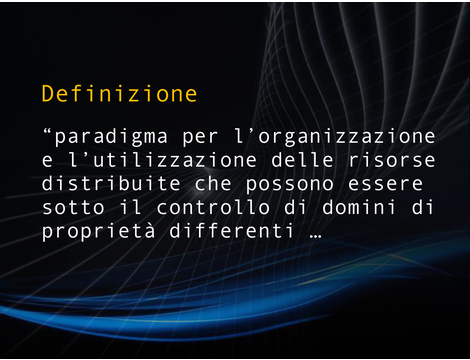
\includegraphics[width=0.50\textwidth,
                    trim=20 80 20 40, % L B R T
                    clip]
                    {images/Lez14_p03_fig_03}
  % \caption{Sommario}
  % \label{fig:Lez15_p06_fig_02}
\end{figure}
\FloatBarrier
\noindent

La Service Orientated Architecture è un paradigma per l'organizzazione e l'utilizzazione delle risorse distribuite che possono essere sotto il controllo di domini di proprietà differenti.

\FloatBarrier
\begin{figure}[H]
  \centering
  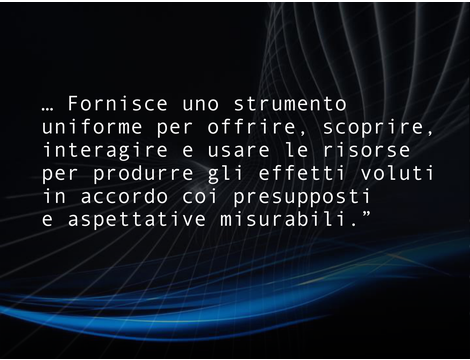
\includegraphics[width=0.50\textwidth,
                    trim=20 80 20 40, % L B R T
                    clip]
                    {images/Lez14_p03_fig_04}
  % \caption{Sommario}
  % \label{fig:Lez15_p06_fig_02}
\end{figure}
\FloatBarrier
\noindent

Inoltre fornisce uno strumento uniforme per offrire, scoprire, interagire e usare le risorse per produrre gli effetti voluti in accordo con i presupposti e aspettative misurabili.

Vediamo che alcuni concetti di questa definizione sono rilevanti.
Innanzitutto stiamo parlando di un paradigma, di un modello, non siamo nell'ambito della tecnologia.
Inoltre le risorse possono essere sotto il controllo di domini di proprietà differenti; questo significa che le risorse possono essere alocalizzate ma soprattutto sotto gestori differenti.

Avremo la possibilità di costruire un modello di calcolo che faccia riferimento a risorse gestite da organizzazioni differenti.

Inoltre il paradigma SOA fornisce uno strumento uniforme; vuol dire che le risorse dovranno comunque essere presentate in una maniera omogenea, in una maniera unitaria orientata alla richiesta dell'utente.

Non abbiamo delle interfacce che ci permettono di accedere in maniera diversa ai vari servizi piuttosto che alle varie applicazioni, piuttosto che ai vari sistemi ma l'accesso dovrà avere una sua uniformità.

\FloatBarrier
\begin{figure}[H]
  \centering
  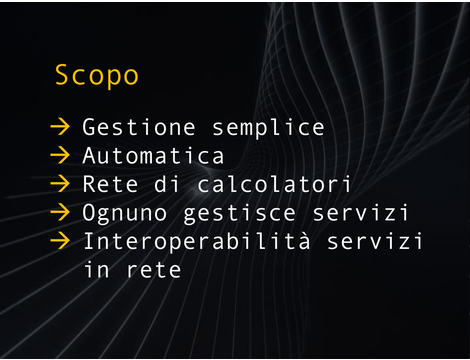
\includegraphics[width=0.50\textwidth,
                    trim=20 60 20 40, % L B R T
                    clip]
                    {images/Lez14_p03_fig_05}
  % \caption{Sommario}
  % \label{fig:Lez15_p06_fig_02}
\end{figure}
\FloatBarrier
\noindent
%%%%%%%%%%%%%%%%%%%%%%%%%%%%%%%%%%%%%%%%%%%%%%%%%%%%%23:45%%%%%%%%%%%%%%%%%%%%%%%%%%%%%%%%%%%%%%%%%%%%%%%%%%%%%%%%%%%%
Lo scopo è molteplice, la gestione semplice, automatica perché altrimenti i tempi di overload gestionale sono eccessivi.

La rete di calcolatori, sono gli attori che intervengono nella realizzazione di questo paradigma, gli esecutori di elementi di applicazioni autonomi.
I calcolatori sono blandamente vincolati, loosely coupled, ognuno conosce la disponibilità delle macchine adiacenti, delle risorse adiacenti, ma non ha controllo sull'esecuzione, non ha controllo gestionale sulle altre macchine.
Ognuno gestisce il servizio o l'insieme di servizi a cui è dedicato sulla base dell'orchestrazione o della coreografia complessiva.

Il fattore basilare è l'interoperabilità dei vari servizi e delle macchine naturalmente, degli attori coinvolti in questa architettura.

\FloatBarrier
\begin{figure}[H]
  \centering
  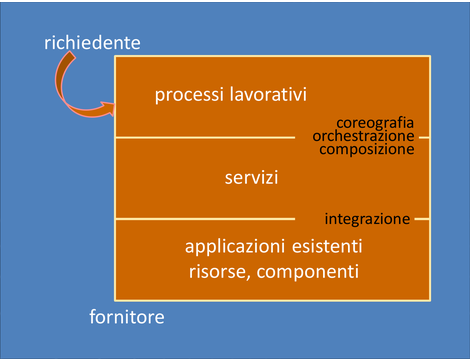
\includegraphics[width=0.50\textwidth,
                    trim=20 20 10 20, % L B R T
                    clip]
                    {images/Lez14_p03_fig_06}
  % \caption{Sommario}
  % \label{fig:Lez15_p06_fig_02}
\end{figure}
\FloatBarrier
\noindent



Vediamo una sintesi grafica.

Il fornitore dispone dell'applicazione o delle risorse.

Il primo livello gestionale è per l'integrazione di queste risorse di calcolo, software, risorse fisiche ma virtualizzate per la composizione di servizi elementari.
I servizi possono essere organizzati come web services, quindi offerti attraverso dei cataloghi con le descrizioni dei servizi e eventualmente composti in servizi più complessi da offrire come attività lavorative utili ai processi lavorativi del richiedente.

La composizione dei servizi è modulata dall'orchestrazione che definisce la regia unica dei servizi selezionati o la coreografia che invece descrive il modo di coordinarsi lasciando autonomia ai servizi o meglio evitando una unica regia nella gestione del processo.

\subsection{Grid Computing}

\FloatBarrier
\begin{figure}[H]
  \centering
  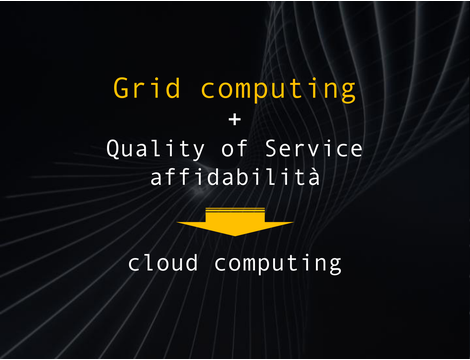
\includegraphics[width=0.50\textwidth,
                    trim=60 60 60 60, % L B R T
                    clip]
                    {images/Lez14_p04_fig_01}
  % \caption{Sommario}
  % \label{fig:Lez15_p06_fig_02}
\end{figure}
\FloatBarrier
\noindent

Un altro concetto rilevante è il grid computing che unitamente alla qualità del servizio e all'affidabilità costituisce il modello cloud computing.
Possiamo dire che il modello che dettaglieremo, riferito come grid computing di organizzazione e di erogazione dei servizi, costituisce il modello cloud computing con strumenti per la garanzia della qualità del servizio e della affidabilità.

Vedremo soprattutto nella parte sugli svantaggi del cloud computing quali siano gli elementi che possano costituire un rischio in questa gestione, economica e molto efficace delle risorse.

\FloatBarrier
\begin{figure}[H]
  \centering
  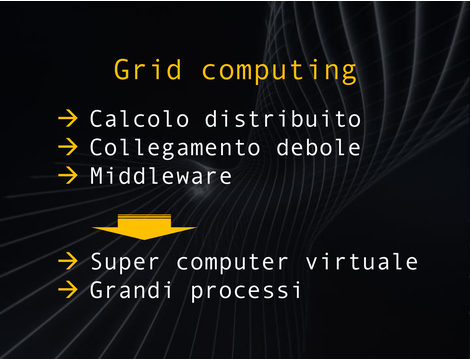
\includegraphics[width=0.50\textwidth,
                    trim=40 40 40 40, % L B R T
                    clip]
                    {images/Lez14_p04_fig_02}
  % \caption{Sommario}
  % \label{fig:Lez15_p06_fig_02}
\end{figure}
\FloatBarrier
\noindent

Il modello grid computing è un modello di calcolo distribuito, fa riferimento a una rete di calcolatori che indica il collegamento topologico, la raggiungibilità di una macchina con l'altra, non il tipo di collegamento locale piuttosto che geografico e neppure la velocità o quali altri caratteristiche tecniche vogliamo dare al tipo di collegamento.

Le unità di calcolo sono tra loro raggiungibili e mantengono un collegamento debole.

Questi modelli di architetturali fanno riferimento ad elementi di calcolo tra loro vincolati da collegamenti deboli.

Anche il grid computing fa riferimento a middleware, a un livello gestionale per il coordinamento delle attività, per l'attivazione degli elementi, delle unità di calcolo necessarie alla conduzione del processo di attualizzazione del servizio.

Questo tipo di gestione che parte da unità di calcolo che possono essere piccole, poco potenti, comunque di capacità molto limitata, permette di organizzare supercomputer virtuali che si presentano come una risorsa di calcolo unitaria, come un unico calcolatore in grado di effettuare grandi processi per quanto riguarda la loro complessità e il loro costo in termini di uso di risorse di calcolo.

\FloatBarrier
\begin{figure}[H]
  \centering
  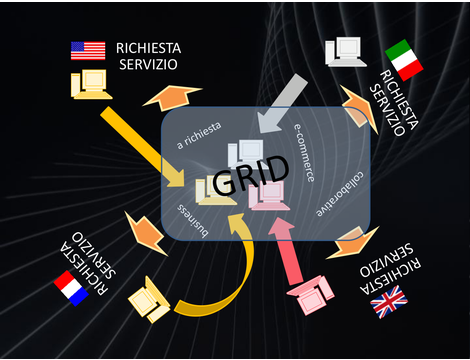
\includegraphics[width=0.50\textwidth,
                    trim=40 20 40 20, % L B R T
                    clip]
                    {images/Lez14_p04_fig_03}
  % \caption{Sommario}
  % \label{fig:Lez15_p06_fig_02}
\end{figure}
\FloatBarrier
\noindent

Vediamo uno schema differente di architettura grid.
Noi rappresentiamo l'ambito di coordinamento di un insieme di risorse, di elementi autonomi poco o blandamente collegati che erogano servizi differenti, una grande varietà di servizi che deve soddisfare richieste che vengono da locazioni non predefinite e comunque indipendenti dal tipo di erogazione del servizio.

L'utente effettua una richiesta di un tipo di servizio e nel modello vengono selezionate le risorse di calcolo che possono sostenere il tipo di servizio che viene richiesto; ogni volta potranno essere selezionate risorse differenti.

\FloatBarrier
\begin{figure}[H]
  \centering
  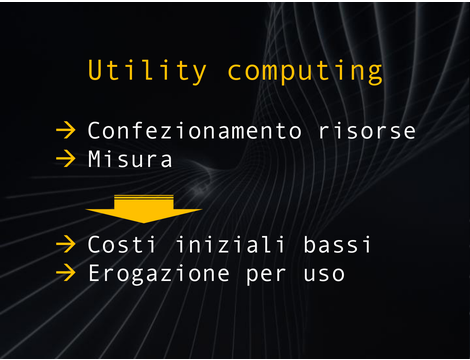
\includegraphics[width=0.50\textwidth,
                    trim=40 40 40 40, % L B R T
                    clip]
                    {images/Lez14_p04_fig_04}
  % \caption{Sommario}
  % \label{fig:Lez15_p06_fig_02}
\end{figure}
\FloatBarrier
\noindent


Vediamo ora il concetto successivo a supporto del modello cloud computing.
Parliamo dell'utility computing, è un modo di confezionamento delle risorse, quindi disponibilità di risorse di calcolo che devono essere selezionate e raggruppate per un obiettivo.
L'utility computing è il fondamento della gestione delle risorse orientata ai servizi che vengono di volta in volta selezionate per quello specifico servizio che le richiede; ma l'utility computing richiede anche un'altra caratteristica, la misura del servizio e della risorsa.

L'utility computing pacchettizza e organizza le risorse necessarie e ne misura il consumo per poter permettere una erogazione di servizi a costi iniziali bassi, in quanto non è necessario con questo tipo di offerta di risorse offrire all'utente l'intera risorsa fisica con lo spreco probabile di una parte.

Inoltre con la misurazione dei servizi e dell'uso delle risorse è possibile un'erogazione sulla base dell'uso, quindi sulla base della quantità richiesta o necessaria all'utente.

\subsection{Compatibilità dei dati}

\FloatBarrier
\begin{figure}[H]
  \centering
  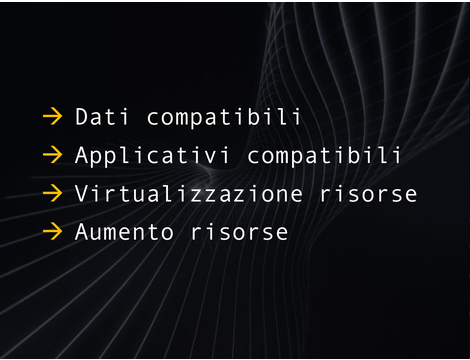
\includegraphics[width=0.50\textwidth,
                    trim=40 80 40 80, % L B R T
                    clip]
                    {images/Lez14_p04_fig_05}
  % \caption{Sommario}
  % \label{fig:Lez15_p06_fig_02}
\end{figure}
\FloatBarrier
\noindent


Inoltre dobbiamo considerare la compatibilità dei dati.
Un problema grosso nelle grandi organizzazioni organizzate in reparti con una certa autonomia operativa è proprio la compatibilità dei dati che viene risolta da questo tipo di gestione  opera affinché vi sia un'interoperabilità almeno sintatica, quindi concernente la formattazione, il tipo di dati, la trasferibilità e l'eventuale confronto e composizione dei dati.

Anche gli applicativi devono essere compatibili, ci riferiamo sempre alla interoperabilità, devono permettere scambio di dati e intendere e interpretare i dati scambiati in maniera  uniforme.

Le risorse sono virtualizzate nel utility computing, quindi abbiamo la potenzialità di usufruire di risorse illimitate rette da una corrispondente risorsa fisica in quel momento limitata.

Questo però permette l'aumento delle risorse, in quanto le risorse virtuali possono essere erogate in ammontare illimitato.

\FloatBarrier
\begin{figure}[H]
  \centering
  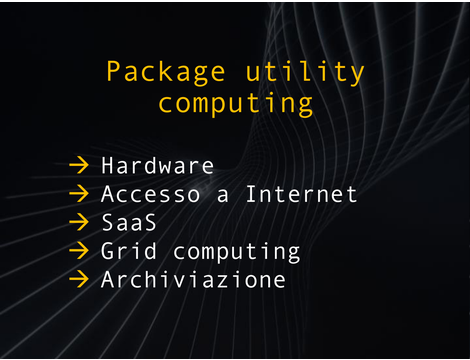
\includegraphics[width=0.50\textwidth,
                    trim=40 40 40 40, % L B R T
                    clip]
                    {images/Lez14_p04_fig_06}
  % \caption{Sommario}
  % \label{fig:Lez15_p06_fig_02}
\end{figure}
\FloatBarrier
\noindent

In questo modello di utility computing una erogazione tipica comprende hardware, accesso a internet, accesso a un collegamento a rete.
Al pacchetto potremo unire l'uso di software applicativi come servizio, quindi erogati attraverso servizi basati sul modello di grid computing o anche accesso a servizi di gestione dei dati come file system condivisi piuttosto che accessi a accesso a basi di dati.

Spunto di riflessione: descrivete i tre concetti computazionali e service oriented che sono connessi al modello cloud, quindi i tre concetti che sono all'origine logica ma anche alla costituzione logica del modello.

\subsection{Svantaggi adozione Cloud Computing}

\FloatBarrier
\begin{figure}[H]
  \centering
  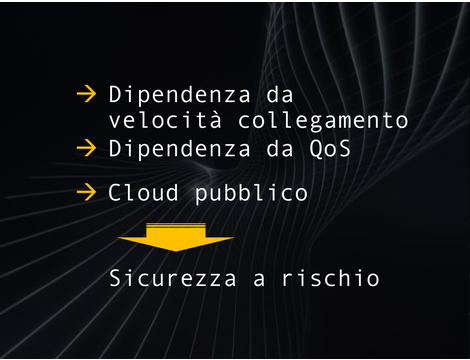
\includegraphics[width=0.50\textwidth,
                    trim=40 40 40 40, % L B R T
                    clip]
                    {images/Lez14_p05_fig_03}
  % \caption{Sommario}
  % \label{fig:Lez15_p06_fig_02}
\end{figure}
\FloatBarrier
\noindent

L'erogazione di questo servizio dipende dalla velocità del collegamento che purtroppo può essere gestita da un provider, da un gestore diverso dal gestore del cloud.

Il servizio dipende fortemente dalla quality of service e si riferisce al collegamento, al rispetto della privacy dei dati, alla protezione da accessi indesiderati e danneggiamento delle procedure o in qualche modo intralcio alla buona conduzione del servizio.

\FloatBarrier
\begin{figure}[H]
  \centering
  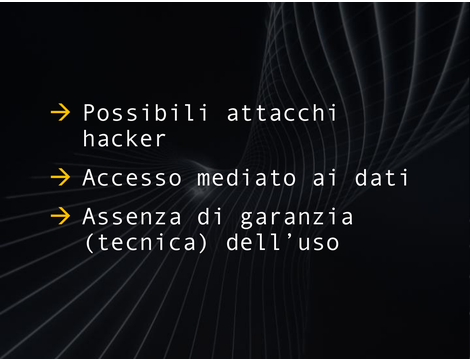
\includegraphics[width=0.50\textwidth,
                    trim=40 60 40 60, % L B R T
                    clip]
                    {images/Lez14_p05_fig_04}
  % \caption{Sommario}
  % \label{fig:Lez15_p06_fig_02}
\end{figure}
\FloatBarrier
\noindent

Un cloud pubblico è molto soggetto a rischi di accessi indesiderati, quindi da possibili attacchi esterni dagli hacker.

Un altro punto da considerare e rigurda la privacy dei dati è la gestione dei diritti, quindi all'accesso lecito e l'uso lecito di questi dati.

Infatti essendo l'accesso mediato da livello di virtualizzazione ma anche da un altro gestore dell'intero servizio, avremo una non completa garanzia dell'uso che viene fatto dei dati e una  assenza di garanzia tecnica dell'uso perché la protezione dei dati può essere non prevenuta ma può essere in qualche modo protetta, ricambiata con contratti, con accordi che prevedano eventualmente penali o costi in caso di danneggiamento.

\FloatBarrier
\begin{figure}[H]
  \centering
  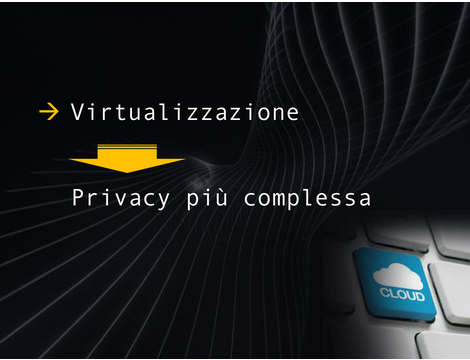
\includegraphics[width=0.50\textwidth,
                    trim=20 100 60 60, % L B R T
                    clip]
                    {images/Lez14_p05_fig_05}
  % \caption{Sommario}
  % \label{fig:Lez15_p06_fig_02}
\end{figure}
\FloatBarrier
\noindent

La virtualizzazione se da una parte rende la gestione molto potente, molto scalabile, dall'altra rende la privacy più complessa  e offre un ulteriore punto di entrata per eventuali accessi di malintenzionati.

\FloatBarrier
\begin{figure}[H]
  \centering
  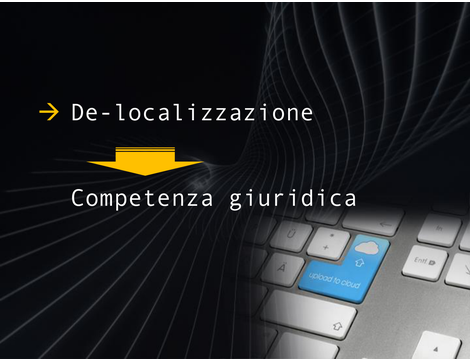
\includegraphics[width=0.50\textwidth,
                    trim=20 100 60 60, % L B R T
                    clip]
                    {images/Lez14_p05_fig_06}
  % \caption{Sommario}
  % \label{fig:Lez15_p06_fig_02}
\end{figure}
\FloatBarrier
\noindent

Altro punto da considerare quale possibile svantaggio del modello è la delocalizzazione delle risorse che può presentare dei problemi per quanto riguarda la competenza giuridica.

Spunti di riflessione: elaborate un esempio di processo lavorativo, servizi al suo supporto, erogati secondo il modello cloud e in conclusione provate a vedere gli svantaggi in questo ambito del modello cloud.
